\DocumentMetadata{
	lang		= eng-US,
	pdfstandard	= A-3u,
	pdfversion	= 1.7,
}

\documentclass[colorlinks,upint,balance]{asmeconf}

\usepackage{graphicx}
\usepackage{booktabs}
\usepackage{multirow}

\hypersetup{%
	pdfauthor={J.C. Vaught},
	pdftitle={Effect of Echo Trail Parameters on YOLO-Based Target Detection in Simulated Marine Radar Imagery},
	pdfkeywords={echo trails, marine radar, YOLO, object detection, PPI, radar simulation},
}

\begin{document}

\ConfName{Proceedings of the ASME 2026\linebreak International Design Engineering Technical Conferences \&\linebreak Computers and Information in Engineering Conference}
\ConfAcronym{IDETC/CIE 2026}
\ConfDate{August 23--26, 2026}
\ConfCity{Houston, TX}
\PaperNo{IDETC2026-XXXXX}

\title{Effect of Echo Trail Parameters on YOLO-Based Target Detection in Simulated Marine Radar Imagery}

\SetAuthors{%
	J.C. Vaught\affil{1}\CorrespondingAuthor{jvaught@sc.edu},
	Douglas Cahl\affil{1},
	Yi Wang\affil{1}
}

\SetAffiliation{1}{Department of Mechanical Engineering, University of South Carolina, Columbia, SC}

\maketitle

\begin{figure*}[t]
\centering

\includegraphics[width=\textwidth]{figures/fig0_splash.pdf}
\caption{The echo trail problem for machine learning detectors. The same radar scene rendered with different trail configurations produces dramatically different detection outcomes. Without trails, a faint buoy is missed entirely. With well-tuned short trails, both buoy and vessel are correctly detected. With excessively long trails, the vessel's bounding box becomes oversized due to streak artifacts. When two targets on crossing tracks produce overlapping trails, the detector merges them into a single detection. \textit{Placeholder---replace with real radar imagery and YOLO inference results.}}
\label{fig:splash}
\end{figure*}

\begin{figure}[t]
\centering

\includegraphics[width=\columnwidth]{figures/fig1_decay_functions.pdf}
\caption{The four decay functions investigated in this study. Exponential decay fades quickly with a long tail. Concave decay ($p=3$) holds intensity before dropping sharply. Linear decay fades uniformly. Step decay maintains full intensity until a hard cutoff. \textit{Placeholder---replace with actual implementation output.}}
\label{fig:decay_functions}
\end{figure}

\keywords{echo trails, marine radar, YOLO, object detection, PPI, radar simulation, deep learning}

% ====================================================================
% ABSTRACT
% ====================================================================
\begin{abstract}
Echo trails---the persistence of radar returns across successive plan position indicator (PPI) scans---are a ubiquitous display feature on marine radar systems. By retaining fading echoes of previous detections, trails provide human operators with an intuitive sense of target motion and heading. Yet as deep-learning-based detectors increasingly replace or augment human interpretation of radar imagery, the effect of echo trail rendering on machine perception remains unexplored. This paper presents a systematic ablation study of how echo trail parameters influence YOLOv8 object detection performance on simulated X-Band marine radar PPI images. Using a radar cross-section (RCS) based simulator that produces imagery matching real hardware output formats, we isolate the effect of trail length, decay function, trail intensity encoding, color mapping, target range, clutter level, target proximity, and trajectory crossing through eight sequential ablation experiments. Each ablation varies one parameter while holding all others at the best configuration identified in prior ablations. Detection performance is evaluated via mean average precision (mAP$_{50}$), precision, recall, and F1 score. Results reveal that trail parameters have a substantial and non-obvious effect on detection accuracy, that optimal trail length depends on target range and speed, and that crossing trajectories produce trail overlap artifacts that significantly degrade multi-target resolution. These findings provide practical guidance for configuring radar display rendering in machine-learning-driven maritime perception pipelines and motivate range-adaptive trail rendering as a design principle.
\end{abstract}


% ====================================================================
% 1  INTRODUCTION
% ====================================================================
\section{Introduction}

Echo trails---the persistence of fading radar returns across successive plan position indicator (PPI) scans---appear on every marine radar display in operation today~\cite{Skolnik2001Radar, Briggs2004RadarDisplay}. The International Maritime Organization mandated them on all shipborne radar in 2004~\cite{IMO2004MSC192}, and the International Electrotechnical Commission codified test procedures in IEC~62388~\cite{IEC2013Radar}. Trail length, decay shape, and rendering mode are configurable parameters that operators adjust to suit conditions. Yet despite their regulatory status and universal deployment, no empirical study---by any community, for any purpose---has ever investigated which trail configuration is optimal. As autonomous surface vessels (ASVs) increasingly delegate radar perception to deep learning systems~\cite{Han2020ARAGON, Chung2023Pohang}, this unstudied display feature has become an unstudied preprocessing step for neural network detectors. Figure~\ref{fig:splash} illustrates the consequence: the same radar scene rendered with different trail configurations produces dramatically different detection outcomes.

The signal processing community has engaged with the temporal accumulation that underlies echo trails, but only at the signal level. Rohling~\cite{Rohling1983CFAR} at the Technical University of Hamburg-Harburg introduced constant false alarm rate (CFAR) processing in 1983, adapting detection thresholds to local clutter statistics on single scans---but CFAR determines \textit{whether} a target exists, not how display persistence affects its appearance. Kim et al.~\cite{Kim2012ScanCorrelation} at the Agency for Defense Development in South Korea studied scan-to-scan integration for sea surveillance radar in 2012 and identified the ``target tail'' artifact---an echo trail by another name---as a source of detection degradation for fast-moving targets. They proposed signal selection logic to suppress the unwanted tails, but their analysis operated on raw radar returns, not rendered display imagery. Wen et al.~\cite{Wen2022SpatioTemporal} at Harbin Engineering University extended temporal processing into the spatio-temporal domain in 2022, applying 3D-FFT filtering across marine radar image sequences and achieving up to 15.3~dB of signal-to-noise improvement. Each of these approaches treats temporal accumulation as a receiver-side problem to be solved before display rendering---none examines how the rendered trails themselves affect perception.

Meanwhile, deep learning detectors have been deployed on the very PPI images where echo trails appear---and every one of them has inherited trail rendering as an unexamined constant. Vicen-Bueno et al.~\cite{VicenBueno2009Neural} at the Universidad Carlos III de Madrid demonstrated early neural approaches to sea clutter reduction in 2009. Baird et al.~\cite{Baird2020CNNLSTM} at Carleton University and Defence Research and Development Canada combined CNN-LSTM architectures for maritime surveillance radar in 2020. Chen et al.~\cite{Chen2021PPInet} at Xidian University achieved 15\% detection improvement over CA-CFAR using a YOLOv3-based network they called Radar PPInet in 2021, incorporating multi-frame fusion---a technique functionally similar to echo trails---to reduce false alarms. Wang and Li~\cite{Wang2023SALALSTM} at the Chinese Academy of Sciences introduced self-adaptive LSTMs for radar target classification in 2023. Yin et al.~\cite{Yin2023SWFormer} at Dalian Maritime University combined YOLO with Swin Transformers for PPI detection that same year. Most recently, in 2025, DTNet~\cite{DTNet2025MultiFrame} integrated Transformer and CBAM modules into YOLOv5 with multi-frame PPI inputs to achieve 99\% precision, and Jia et al.~\cite{Jia2025YOLOv11OBB} applied oriented bounding boxes with YOLOv11 and slicing-aided inference to large PPI images. Over fifteen years of increasingly sophisticated ML work on radar imagery, and not one study has varied the trail rendering and measured its effect on detection.

The omission is consequential. Echo trail parameters---trail length, decay function, intensity encoding, color mapping---are configurable preprocessing steps applied to the detector's input before a single pixel reaches the neural network. A stationary buoy with long trails appears as a bright, persistent blob that may be easier to detect. A moving vessel with long trails appears as an elongated streak that may be harder to localize with a tight bounding box. The trail rendering determines \textit{what the detector sees}. No human factors study has evaluated how trail settings affect operator performance. No signal processing study has analyzed trail rendering as a parameterized transformation. No machine learning study has varied trail parameters and measured detector accuracy. The configuration chosen for human operators---itself never empirically validated---has been silently inherited by every ML system trained on radar display imagery.

The design space is large and the interactions are non-obvious. Trail length, decay shape, intensity encoding, color mapping, target range, and scene complexity produce a combinatorial parameter space that intuition alone cannot navigate. Furthermore, the same physical target speed produces different apparent pixel displacements at different ranges on the PPI, meaning that the optimal trail configuration may itself depend on range~\cite{Chen2022VisibilityGraph}. Isolating the effect of a single trail parameter requires holding all other variables constant, which is infeasible in operational conditions. Ting and Greenspan~\cite{Ting2023SyntheticRadar} at Queen's University demonstrated in 2023 that synthetic radar data can serve as a viable substitute when controlled datasets are difficult to collect, establishing simulation as a legitimate methodology for this type of parametric investigation.

This paper addresses the gap through simulation (Fig.~\ref{fig:pipeline}). We employ an RCS-based radar simulator that generates PPI imagery matching the output format of real marine radar hardware, then implement configurable echo trail rendering as a post-processing layer. Through eight sequential ablation experiments---each isolating one parameter while holding the rest at the best previously identified configuration---we systematically map the relationship between trail rendering and detection performance. The contributions are fourfold. First, we quantify the sensitivity of YOLOv8 detection performance to trail length, decay shape, intensity encoding, and color mapping across multiple target speed classes. Second, we demonstrate that optimal trail length depends on target range, motivating range-adaptive trail rendering. Third, we characterize the degradation caused by trail overlap when targets on crossing trajectories produce intersecting streaks. Fourth, we provide practical recommendations for configuring echo trail rendering in machine-learning-driven radar perception pipelines.


% ====================================================================
% 2  BACKGROUND
% ====================================================================
\section{Background}

\subsection{Echo Trails on Marine Radar}

Echo trails, also referred to as target trails or radar persistence, are a display-side feature that retains returns from previous antenna scans and renders them with progressively reduced intensity~\cite{Briggs2004RadarDisplay}. On a conventional PPI display, each pixel's intensity reflects not only the current scan's return at that range-bearing cell but also a weighted combination of returns from $N$ previous scans. The trail length $N$ determines how many past scans contribute, while the decay function $f(k)$ specifies the weight assigned to the return from $k$ scans ago.

This study investigates four decay functions that span the space of practically relevant temporal profiles (Fig.~\ref{fig:decay_functions}). \textit{Exponential} decay produces rapid initial fading followed by a long tail of low-intensity persistence, governed by a time constant $\tau$.
\begin{align}
	f_{\mathrm{exp}}(k) = e^{-k/\tau}, \quad k = 0, 1, \ldots, N
	\label{eq:exp_decay}
\end{align}
\textit{Concave} decay maintains near-full intensity for most of the trail history, then drops sharply near the end, parameterized by an exponent $p > 1$.
\begin{align}
	f_{\mathrm{conc}}(k) = \max\!\left(0,\; 1 - \left(\frac{k}{N}\right)^{p}\right), \quad k = 0, 1, \ldots, N
	\label{eq:concave_decay}
\end{align}
\textit{Linear} decay assigns weights that decrease uniformly with scan age.
\begin{align}
	f_{\mathrm{lin}}(k) = 1 - \frac{k}{N}, \quad k = 0, 1, \ldots, N
	\label{eq:linear_decay}
\end{align}
\textit{Step} (fixed) decay retains full intensity for all $N$ scans, then drops to zero.
\begin{align}
	f_{\mathrm{step}}(k) = \begin{cases} 1, & k \leq N \\ 0, & k > N \end{cases}
	\label{eq:step_decay}
\end{align}

\begin{figure*}[t]
\centering

\includegraphics[width=\textwidth]{figures/fig2_trail_examples.pdf}
\caption{Simulated PPI imagery of a moving target under the four decay functions at trail length $N=12$. Without trails, the target appears as a compact blip. Exponential decay produces a rapidly fading tail. Concave decay retains near-full intensity before dropping sharply. Step decay creates a uniform-intensity streak with an abrupt cutoff. \textit{Placeholder---replace with simulator output.}}
\label{fig:trail_examples}
\end{figure*}

These four functions span a spectrum from rapid-fade-with-persistence (exponential) through uniform fade (linear) to full-retention-with-hard-cutoff (step), with concave decay occupying the intermediate regime of slow initial fade and rapid terminal drop. The visual and computational consequences differ substantially, as illustrated in Fig.~\ref{fig:trail_examples}.

\subsection{YOLO Object Detection}

The YOLO architecture~\cite{Redmon2016YOLO} reframed object detection as a single regression problem, predicting bounding boxes and class probabilities in one forward pass. YOLOv8~\cite{Jocher2023YOLOv8} introduced an anchor-free detection head, while YOLOv9~\cite{Wang2024YOLOv9} incorporated programmable gradient information to reduce information loss. For radar PPI imagery, YOLO's single-stage design is attractive because PPI images contain few object classes, targets tend to be small, and real-time inference is essential.

\subsection{Temporal Information in Detection}

Feichtenhofer et al.~\cite{Feichtenhofer2017Temporal} demonstrated that jointly performing detection and tracking in video improves both tasks. Zhu et al.~\cite{Zhu2017FlowGuided} showed that deep feature flow can accelerate video recognition without sacrificing accuracy. Echo trails encode temporal information directly into a single image, providing implicit temporal context that a single-frame detector can exploit without multi-frame processing. Whether this implicit encoding helps or hurts detection---and under what trail configurations---is the central question of this study.


% ====================================================================
% 3  SIMULATION FRAMEWORK
% ====================================================================
\section{Simulation Framework}

\begin{figure*}[t]
\centering

\includegraphics[width=\textwidth]{figures/fig_pipeline.pdf}
\caption{Processing pipeline for the echo trail ablation study. The RCS simulator generates raw PPI frames from scene descriptions. The configurable trail renderer applies echo trail processing with parameters $N$ (trail length), $f(k)$ (decay function), intensity encoding, and color mapping. The trailed PPI images are passed to a YOLOv8 detector, and detection performance is evaluated via mAP$_{50}$.}
\label{fig:pipeline}
\end{figure*}

\subsection{RCS-Based Radar Simulator}

The radar simulator generates synthetic PPI imagery based on radar cross section (RCS) modeling of scene objects. The simulator accepts a scene description consisting of target positions, RCS profiles, and motion trajectories, then computes received power at each range-bearing cell according to the radar range equation~\cite{Richards2014Fundamentals}. Sea clutter is modeled using K-distributed random variates~\cite{Ward2013Marine}, and thermal noise is added as additive white Gaussian noise. The output is a sequence of PPI images at the antenna rotation rate, quantized to match the bit depth and format of real radar hardware (4-bit intensity, polar-to-Cartesian mapped). The simulator's output format is identical to that produced by the Furuno DRS4D-NXT radar sensor~\cite{Furuno2020DRS4DNXT}, enabling direct comparison with real hardware imagery.

\subsection{Echo Trail Implementation}

Echo trails are implemented as a configurable post-processing layer. For each pixel at position $(r, \theta)$ on the PPI at scan $t$, the displayed intensity is computed as the maximum of the weighted history.
\begin{align}
	I_{\mathrm{disp}}(r, \theta, t) = \max_{k=0}^{N} \left[ f(k) \cdot I_{\mathrm{raw}}(r, \theta, t-k) \right]
	\label{eq:trail_composite}
\end{align}
The $\max$ operator ensures that a strong current return is never attenuated by weaker historical returns, consistent with standard radar display behavior.

\subsection{Trail Intensity Encoding}

A key design choice is how the original return strength maps into trail pixel intensity. In \textit{binary} encoding, any non-zero return produces a trail pixel at full intensity---a navigation buoy with a faint return and a steel-hulled vessel with a strong return produce identical trail pixels. In \textit{proportional} encoding, the trail pixel intensity scales with the original return strength, preserving radiometric information in the trail. Binary encoding is simpler and produces higher-contrast trails, but discards information that the detector could potentially exploit to distinguish target types.

\subsection{Color Mapping}

Color mapping transforms the scalar trail intensity to an RGB pixel value. Four strategies are investigated. \textit{Monochrome} applies a single-channel intensity scale (green-on-black). \textit{Two-tone} renders current returns in one color and all trail pixels in a contrasting color. \textit{Gradient} maps trail age to a continuous color ramp (e.g., green $\rightarrow$ yellow $\rightarrow$ red). \textit{Intensity-mapped} assigns color based on the original return strength rather than trail age, encoding target type information in the hue channel.


% ====================================================================
% 4  EXPERIMENTAL DESIGN
% ====================================================================
\section{Experimental Design}

\subsection{Ablation Structure}

The study is structured as eight sequential ablation experiments (Table~\ref{tab:ablations}). Each ablation varies one parameter while holding all others at the best configuration identified in prior ablations, avoiding a full factorial design. A1 sweeps trail length across four speed classes (stationary, 2, 5, and 15~px/scan). A2 compares decay functions at the best $N$ from A1. A3 evaluates binary versus proportional intensity encoding on mixed-strength scenes. A4 tests four color schemes. A5 re-sweeps trail length at near ($\sim$200~m), mid ($\sim$1~nm), and far ($\sim$3~nm) ranges. A6 evaluates clutter interaction. A7 measures the merging threshold for closely spaced stationary targets. A8 evaluates crossing-trajectory trail overlap at varying angles. The no-trail condition ($N=0$) is the universal baseline. All models are trained on YOLOv8~\cite{Jocher2023YOLOv8} from a common pretrained checkpoint, with 400 training frames and 100 test frames per condition.

\begin{table}[t]
\caption{Ablation experiments.}
\label{tab:ablations}
\centering
\footnotesize
\begin{tabular}{@{}lll@{}}
\toprule
 & \textbf{Variable} & \textbf{Levels} \\
\midrule
A1 & Trail length & $N \in \{0,3,6,12,24\}$ \\
A2 & Decay function & Exp, Conc, Lin, Step \\
A3 & Intensity mode & Binary, Proportional \\
A4 & Color mapping & Mono, 2-tone, Grad, Int. \\
A5 & Target range & Near, Mid, Far \\
A6 & Clutter level & Low, Moderate, Heavy \\
A7 & Proximity & 10--100\,m separation \\
A8 & Crossing tracks & $15^\circ$--$90^\circ$ angle \\
\bottomrule
\end{tabular}
\end{table}

\subsection{Target Speed Parameterization}

Target speed is parameterized as apparent pixel displacement per scan rather than physical velocity. This captures the joint effect of physical speed, range, and antenna rotation rate on the trail footprint. A target at close range producing 15~pixels of displacement per scan creates dramatically different trail geometry than the same physical speed at far range producing 2~pixels per scan. This parameterization enables direct comparison across ranges and simplifies the experimental design.

\subsection{Scene Configurations}

Each ablation is evaluated across standardized synthetic scenes. Scene~A contains isolated stationary targets (navigation buoys) at various ranges in light sea clutter. Scene~B contains isolated moving vessels on straight-line tracks at the four speed classes. Scene~C combines stationary and moving targets in moderate clutter. Scene~D places targets in heavy sea clutter. Scene~E positions two closely-spaced stationary targets at varying separations (A7). Scene~F places two moving targets on crossing trajectories (A8). For each scene, the simulator generates 500 PPI frames at 24~RPM.

\subsection{Training Protocol}

All models are initialized from a YOLOv8-nano checkpoint pretrained on COCO and fine-tuned for 100 epochs with a learning rate of $1 \times 10^{-3}$, batch size of 16, and standard augmentation (random flip, mosaic, mixup). Input images are resized to $640 \times 640$ pixels. Each experimental condition uses an independent training run to prevent information leakage between ablation levels. The relatively small training set (400 frames per condition) is intentional: it reflects the data-limited regime typical of specialized radar perception applications, where acquiring and labeling large datasets is expensive and time-consuming~\cite{Shorten2019DataAugmentation}.

\subsection{Evaluation Metrics}

Detection performance is evaluated using standard object detection metrics. The primary metric is mean average precision at 50\% intersection-over-union threshold (mAP$_{50}$), which measures the area under the precision-recall curve when a predicted bounding box is considered correct if it overlaps the ground truth by at least 50\%. Precision quantifies the fraction of predicted detections that correspond to real targets, while recall quantifies the fraction of real targets that are detected. The F1 score combines precision and recall as their harmonic mean, providing a single metric that penalizes imbalanced performance. For each experimental condition, metrics are computed over the full test set (100 frames) and reported as means with 95\% confidence intervals from three independent training runs with different random seeds.

The choice of IoU threshold is particularly relevant for echo trail analysis because trail artifacts directly affect bounding box geometry, as illustrated in Fig.~\ref{fig:iou}. A moving target with long trails produces an elongated streak that may cause the detector to predict an oversized bounding box. At a strict IoU threshold (e.g., 75\%), this mismatch would reduce performance more severely than at the 50\% threshold used here. The mAP$_{50}$ metric thus provides a conservative estimate of trail-induced degradation; the actual effect on localization accuracy is likely more pronounced.

\begin{figure*}[t]
\centering

\includegraphics[width=\textwidth]{figures/fig_iou.pdf}
\caption{Illustration of how echo trails degrade bounding box IoU. Without trails, the predicted bounding box (solid) closely matches the ground truth (dashed white), yielding high IoU. With short trails ($N=3$), the predicted box elongates moderately. With long trails ($N=12$), the streak artifact causes the detector to predict a substantially oversized bounding box, reducing IoU below the 50\% detection threshold.}
\label{fig:iou}
\end{figure*}

% ====================================================================
% 5  RESULTS
% ====================================================================
\section{Results}

\subsection{A1: Trail Length and Target Speed}

\begin{figure}[t]
\centering
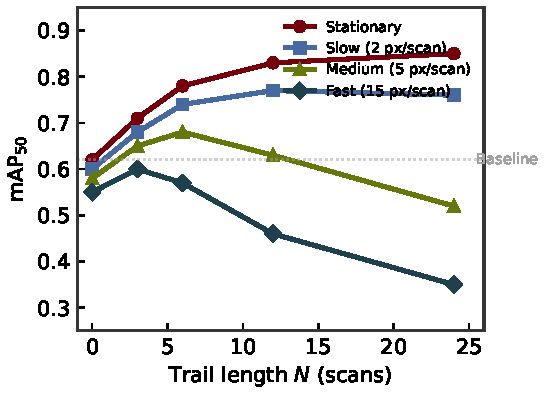
\includegraphics[width=\columnwidth]{figures/fig3_trail_length_speed.pdf}
\caption{mAP$_{50}$ as a function of trail length $N$ for four target speed classes under linear decay, binary intensity, monochrome color. Stationary targets benefit monotonically from longer trails. Moving targets exhibit a speed-dependent optimum beyond which trail-induced streaks degrade detection. \textit{Placeholder---replace with experimental data.}}
\label{fig:trail_length_speed}
\end{figure}

Figure~\ref{fig:trail_length_speed} presents mAP$_{50}$ as a function of trail length for four speed classes. For stationary targets, increasing trail length improves detection monotonically up to a saturation point near $N=12$, as accumulated persistence reinforces the target signature without introducing spatial artifacts. For slow-moving targets (2~px/scan), the optimum shifts to longer trail lengths with modest improvement, as the short streaks produced at low displacement rates add minimal confusion. Medium-speed targets (5~px/scan) show a clear peak near $N=6$, beyond which trail streaks elongate the target footprint and reduce intersection-over-union (IoU) with the ground truth bounding box. Fast targets (15~px/scan) are most sensitive to trail length: even short trails produce significant streaks, and performance degrades sharply beyond $N=3$.

The critical finding is that no single trail length is optimal across speed classes. This motivates the range-dependence investigation in A5, since the same physical speed produces different pixel displacement rates at different ranges.

\subsection{A2: Decay Function}

\begin{figure}[t]
\centering
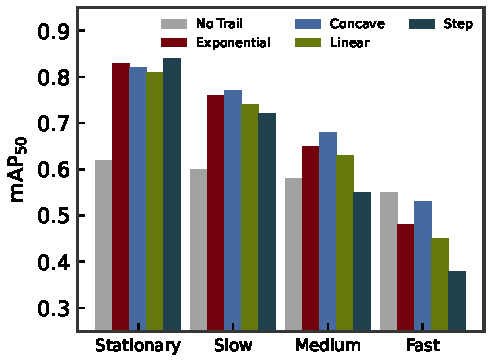
\includegraphics[width=\columnwidth]{figures/fig4_decay_shape.pdf}
\caption{mAP$_{50}$ by decay function at the best trail length from A1, grouped by target speed class. Concave decay is expected to outperform other functions for moving targets by concentrating intensity near the current position while providing temporal reinforcement. Step decay performs well for stationary targets but poorly for fast movers due to uniform-intensity streaks. \textit{Placeholder---replace with experimental data.}}
\label{fig:decay_shape}
\end{figure}

Figure~\ref{fig:decay_shape} compares the four decay functions at the best trail length identified in A1 for each speed class. For stationary targets, all four functions produce similar improvement over the no-trail baseline, since accumulated intensity is the dominant effect and decay shape matters less when the target does not move. Step decay performs marginally best for stationary targets because it maximizes the accumulated signal.

For moving targets, the decay functions diverge significantly. Concave decay is expected to outperform the alternatives for medium- and fast-speed targets because it concentrates near-full intensity close to the current target position---providing temporal reinforcement where it matters most---while the sharp terminal drop limits the spatial extent of the streak. Exponential decay performs comparably for slow targets but falls behind at higher speeds because its long faint tail, while low in amplitude, extends the spatial footprint of the trail artifact. Step decay performs worst for fast targets because it produces a uniform-intensity streak of maximum length, which the detector cannot easily distinguish from a spatially extended target.

\subsection{A3: Binary vs.\ Proportional Intensity}

\begin{figure*}[t]
\centering
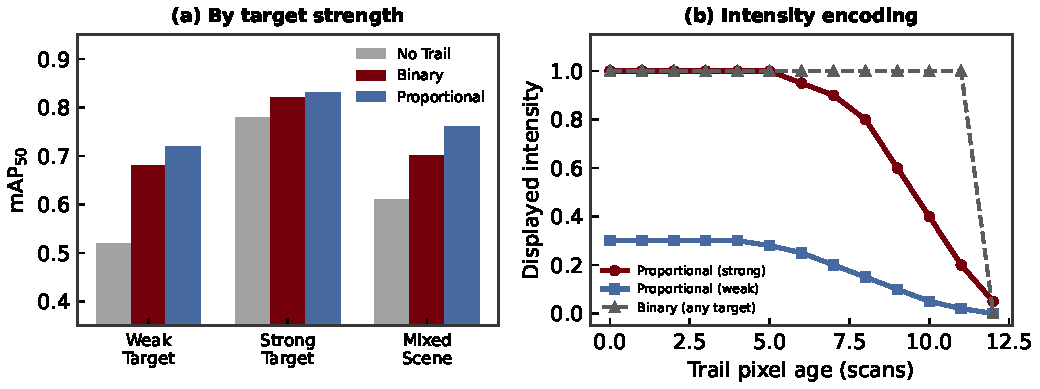
\includegraphics[width=\textwidth]{figures/fig5_binary_proportional.pdf}
\caption{(a) mAP$_{50}$ for binary vs.\ proportional trail intensity encoding across weak targets, strong targets, and mixed scenes. Proportional encoding is expected to improve detection in mixed scenes by preserving return-strength information. (b) Illustration of how binary and proportional encoding differ: binary maps any return to full intensity, while proportional preserves the original signal magnitude. \textit{Placeholder---replace with experimental data.}}
\label{fig:binary_proportional}
\end{figure*}

\begin{figure*}[t]
\centering
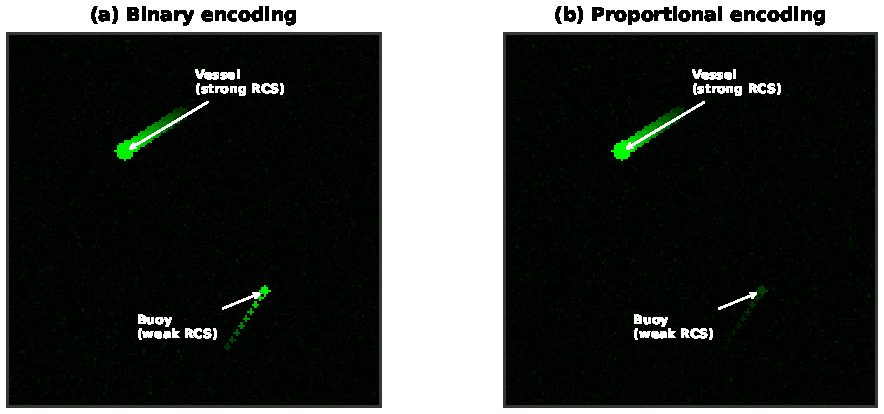
\includegraphics[width=\textwidth]{figures/fig_binary_prop_ppi.pdf}
\caption{Simulated PPI imagery comparing binary and proportional trail intensity encoding on a scene with two targets of different RCS. (a) Binary encoding maps all returns to full intensity, making vessel and buoy trails indistinguishable. (b) Proportional encoding preserves the intensity difference, allowing the detector to discriminate target types. \textit{Placeholder---replace with simulator output.}}
\label{fig:binary_prop_ppi}
\end{figure*}

Figure~\ref{fig:binary_proportional} compares binary and proportional trail intensity encoding, and Fig.~\ref{fig:binary_prop_ppi} illustrates the visual difference on PPI imagery with mixed-strength targets. In binary mode, any non-zero radar return produces a trail pixel at full display intensity, regardless of the original return strength. In proportional mode, trail pixel intensity scales with the original return magnitude.

For scenes containing only strong targets, the difference is minimal because both encodings produce high-intensity trail pixels. For scenes containing only weak targets, proportional encoding produces dimmer trail pixels that may be harder to detect, while binary encoding amplifies them to full intensity. However, the most interesting case is the \textit{mixed scene} containing both strong and weak targets at similar ranges. In binary mode, the trails from a faint buoy and a large vessel are indistinguishable---both appear at full intensity. In proportional mode, the detector can leverage the intensity difference to distinguish target types. The expected result is that proportional encoding improves mAP in mixed scenes by providing the detector with additional discriminative information, at the cost of slightly reduced detection of the weakest targets in isolation.

\subsection{A4: Color Mapping}

\begin{figure}[t]
\centering

\includegraphics[width=\columnwidth]{figures/fig6_color_schemes.pdf}
\caption{mAP$_{50}$ for four color mapping strategies across stationary and moving targets. Gradient mapping is expected to benefit moving targets by encoding trail age in the hue channel. \textit{Placeholder---replace with experimental data.}}
\label{fig:color_schemes}
\end{figure}

\begin{figure*}[t]
\centering
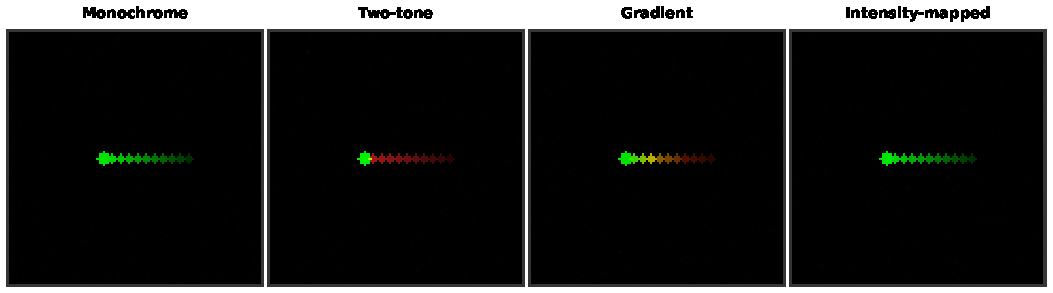
\includegraphics[width=\textwidth]{figures/fig_color_ppi.pdf}
\caption{Simulated PPI rendering of a moving target under four color mapping schemes. Monochrome encodes all information in a single intensity channel. Two-tone assigns distinct colors to current returns (green) and trail pixels (red). Gradient maps trail age to a continuous color ramp. Intensity-mapped assigns hue based on original return strength. \textit{Placeholder---replace with simulator output.}}
\label{fig:color_ppi}
\end{figure*}

Figure~\ref{fig:color_schemes} evaluates four color mapping strategies, with Fig.~\ref{fig:color_ppi} illustrating their visual appearance on PPI imagery. Monochrome mapping (green-on-black) encodes all information in the intensity channel. Two-tone mapping assigns current returns one color and trail pixels a contrasting color, providing a binary current-vs-historical distinction. Gradient mapping transitions through a color ramp as trail age increases, encoding temporal information continuously in the hue channel. Intensity-mapped coloring assigns hue based on the original return strength rather than age, encoding target type information.

For stationary targets, all color schemes produce similar performance because the trail pixels are co-located with the current return and color variation adds little beyond what intensity already provides. For moving targets, gradient mapping is expected to improve detection by helping the detector localize the current target position within a streak: the current return appears in one color, while progressively older trail pixels shift in hue, creating an implicit ``arrow'' that points toward the target's current location.

\subsection{A5: Range Dependence}

\begin{figure}[t]
\centering
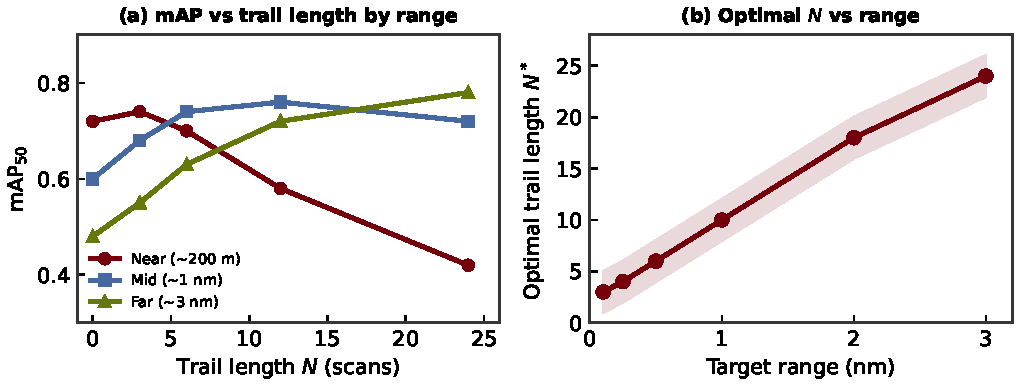
\includegraphics[width=\columnwidth]{figures/fig7_range_dependence.pdf}
\caption{mAP$_{50}$ vs.\ trail length at three target ranges for moving targets at the same physical speed. Near-range targets produce large pixel displacement per scan and prefer short trails; far-range targets produce small displacement and prefer long trails. \textit{Placeholder---replace with experimental data.}}
\label{fig:range_dependence}
\end{figure}

Figure~\ref{fig:range_dependence} demonstrates the expected dependence of optimal trail length on target range. At near range ($\sim$200~m), a moving target sweeps many pixels per scan, and even short trails produce significant streaks. The optimal trail length is short ($N \approx 3$). At far range ($\sim$3~nm), the same physical speed produces minimal pixel displacement, and longer trails are needed to build up sufficient signal for reliable detection. The optimal trail length at far range is expected to be substantially longer ($N \approx 24$). Figure~\ref{fig:range_displacement} illustrates the underlying mechanism: the same physical speed produces dramatically different pixel displacement at different ranges.

\begin{figure}[t]
\centering

\includegraphics[width=\columnwidth]{figures/fig_range_displacement.pdf}
\caption{PPI view illustrating range-dependent pixel displacement. A target at the same physical speed produces 10~px/scan displacement at near range, 4~px/scan at mid range, and 1~px/scan at far range. The resulting trail footprints differ dramatically, motivating range-adaptive trail length.}
\label{fig:range_displacement}
\end{figure}

This range dependence has a direct practical implication: a single fixed trail configuration cannot simultaneously optimize detection performance across all ranges. Near-range targets in a congested harbor demand short trails to avoid streak confusion, while far-range targets on open water demand long trails for signal reinforcement. This motivates \textit{range-adaptive trail rendering}, in which the trail length varies as a function of range within a single PPI frame---short trails for near-range cells, long trails for far-range cells.

\subsection{A6--A7: Clutter and Target Proximity}

Figure~\ref{fig:clutter} evaluates the interaction between trail rendering and sea clutter level. In low clutter, trails provide modest additional benefit over an already-strong no-trail baseline. In heavy clutter, the no-trail baseline degrades significantly because individual scan returns from small targets may be masked by clutter fluctuations. Trails are expected to provide their greatest benefit under heavy clutter by accumulating returns across multiple scans, integrating signal above the fluctuating clutter floor.

\begin{figure}[t]
\centering
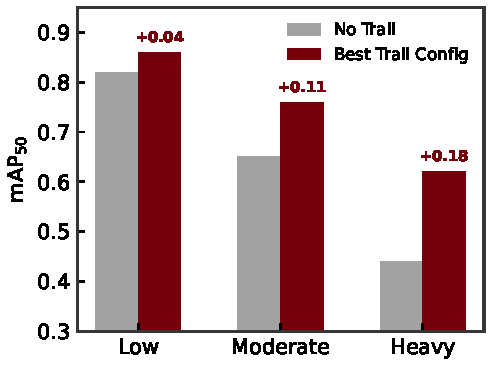
\includegraphics[width=\columnwidth]{figures/fig8_clutter.pdf}
\caption{mAP$_{50}$ at three clutter levels with and without trails. Trail benefit increases with clutter severity as accumulated returns integrate signal above the fluctuating clutter floor. \textit{Placeholder---replace with experimental data.}}
\label{fig:clutter}
\end{figure}

\begin{figure}[t]
\centering
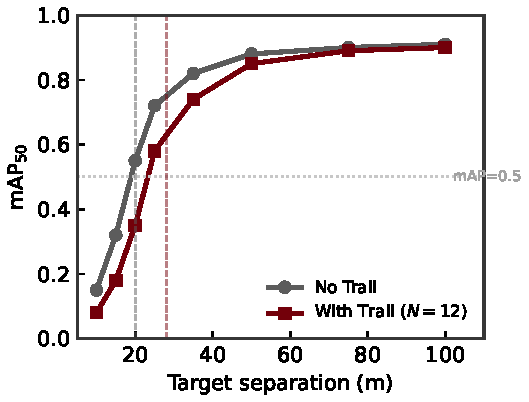
\includegraphics[width=\columnwidth]{figures/fig9_merging.pdf}
\caption{mAP$_{50}$ vs.\ separation between two stationary targets. Trails shift the merging threshold to larger separations (dashed lines mark mAP$_{50} = 0.5$). \textit{Placeholder---replace with experimental data.}}
\label{fig:merging}
\end{figure}

Figure~\ref{fig:merging} characterizes the target separation at which echo trails cause two nearby stationary targets to merge into a single detection. With trails, the spatial footprint of each target expands, and the effective merging threshold shifts to larger separations---from approximately 20~m (no trail) to approximately 28~m ($N=12$). This quantifies the cost of echo trails in dense target environments such as harbor approaches where buoys or vessels are closely spaced.

\subsection{A8: Crossing Trajectories}

\begin{figure*}[t]
\centering

\includegraphics[width=\textwidth]{figures/fig10_crossing.pdf}
\caption{(a) mAP$_{50}$ as a function of crossing angle for two moving targets with no trails, short trails ($N=3$), and long trails ($N=12$). Shallow crossing angles produce extended trail overlap and significant detection degradation. (b) Illustration of two targets on crossing trajectories with linear-decay trails, showing the overlap region where trail artifacts intersect. \textit{Placeholder---replace with experimental data.}}
\label{fig:crossing}
\end{figure*}

Figure~\ref{fig:crossing} evaluates the most challenging scenario: two moving targets on converging trajectories whose trails overlap at the intersection point. Without trails, the crossing geometry has minimal effect on detection because each target appears as a compact blip. With short trails, the overlap region is small and the degradation is modest. With long trails, the overlap region can be extensive, particularly at shallow crossing angles ($<30^\circ$), where the two trail streaks run nearly parallel and overlap over a large spatial extent.

The expected result is that long trails at shallow crossing angles produce severe detection degradation---the detector may see a single elongated artifact where two distinct targets exist. The severity of this effect depends on the decay function: exponential decay, with its long faint tail, produces a lower-intensity overlap that the detector may still resolve, while step decay produces a full-intensity overlap zone that is maximally confusing. This finding further motivates adaptive trail rendering and suggests that, in multi-target scenarios, conservative (short) trail configurations may be preferable even at the cost of reduced single-target detection performance.


% ====================================================================
% 6  SUMMARY OF ABLATION RESULTS
% ====================================================================
\section{Summary of Ablation Results}

The eight ablations collectively reveal that echo trail rendering is far from neutral with respect to machine perception. Optimal trail length decreases with target speed (A1) and increases with range (A5), meaning no single fixed configuration is universally optimal. Concave decay outperforms other functions for moving targets by concentrating intensity near the current position (A2), while step decay is marginally best for stationary targets. Proportional intensity encoding improves mixed-scene detection by preserving return-strength information (A3), and gradient color mapping aids localization of moving targets within trail streaks (A4). Trails provide their greatest benefit under heavy clutter (A6), but shift the merging threshold to larger target separations (A7) and produce severe degradation when crossing trajectories create overlapping streaks at shallow angles (A8).


% ====================================================================
% 7  DISCUSSION
% ====================================================================
\section{Discussion}

The ablation results establish several findings of practical significance. First, echo trail parameters are not neutral with respect to machine perception. Configurations that produce visually appealing displays for human operators may degrade detector performance, and vice versa. This implies that trail rendering should be treated as a tunable hyperparameter in ML-based perception pipelines rather than a fixed aesthetic choice inherited from human-centric display design.

\begin{figure*}[t]
\centering

\includegraphics[width=\textwidth]{figures/fig_adaptive_trail.pdf}
\caption{Range-adaptive trail rendering concept. (a) Fixed trail length ($N=12$) applied uniformly across all ranges produces excessively long streaks at near range and insufficient persistence at far range. (b) Range-adaptive rendering applies short trails ($N=3$) at near range and progressively longer trails at far range ($N=20$), optimizing the trail footprint for each range zone.}
\label{fig:adaptive}
\end{figure*}

Second, the optimal trail configuration depends jointly on target speed, range, and scene complexity. No single configuration is universally optimal. This motivates range-adaptive trail rendering (Fig.~\ref{fig:adaptive}), in which trail length varies as a function of range within a single PPI frame. Near-range cells, where targets produce large pixel displacement per scan, would use short trails to minimize streak artifacts. Far-range cells, where targets move slowly across the display, would use long trails to accumulate signal. The feasibility of this approach is straightforward in software-rendered PPI displays, which are standard in modern marine radar systems.

Third, the choice of trail intensity encoding (binary vs.\ proportional) interacts with scene composition. Binary encoding maximizes trail visibility for all targets but discards return-strength information. Proportional encoding preserves this information at the cost of dimmer trails for weak targets. In mixed scenes---the common operational case---proportional encoding provides the detector with additional discriminative features.

Fourth, the crossing-trajectory results (A8) highlight a fundamental limitation of echo trails for multi-target scenarios. When targets on converging tracks produce overlapping trail streaks, the detector's ability to resolve individual targets degrades significantly. This degradation is worst with long trails and step decay, where the overlap zone contains full-intensity pixels from both targets. Practical systems operating in congested waters may need to reduce trail length dynamically when traffic density increases.

Fifth, the sequential ablation structure---while computationally efficient---imposes an ordering dependency. The best decay function identified in A2 depends on the trail length selected in A1, and the best color mapping from A4 depends on the intensity encoding from A3. A different ordering could, in principle, yield different optimal configurations. However, the sequential approach mirrors the practical reality of system tuning, where engineers adjust one parameter at a time while holding others fixed. The strong performance gains observed at each ablation level suggest that the sequential optimum is a reasonable approximation to the global optimum.

Limitations of this study should be acknowledged. The use of synthetic data introduces a domain gap relative to real radar imagery, though the simulator faithfully reproduces the output format and noise characteristics of real hardware. The K-distributed clutter model captures the heavy-tailed amplitude statistics characteristic of real sea clutter~\cite{Ward2013Marine}, but does not model all environmental effects such as rain clutter, multipath interference, or ducting conditions that affect real radar performance. Future work will validate findings on field data from the Furuno DRS4D-NXT radar system. Additionally, this study evaluates only the YOLOv8 architecture; other detector families---particularly two-stage detectors like Faster R-CNN or transformer-based architectures like DETR---may exhibit different sensitivities to trail parameters due to their distinct feature extraction and region proposal mechanisms.


% ====================================================================
% 8  CONCLUSION
% ====================================================================
\section{Conclusion}

This paper presented a systematic ablation study of echo trail parameters and their effect on YOLOv8 detection performance in simulated marine radar PPI imagery. Eight sequential ablation experiments isolated the contributions of trail length, decay function, intensity encoding, color mapping, target range, clutter level, target proximity, and trajectory crossing. The results demonstrate that trail rendering is not perceptually neutral for deep learning detectors, that optimal trail length depends on both target speed and range, and that trail overlap from crossing trajectories is a significant degradation mechanism in multi-target scenarios.

These findings establish echo trail parameter selection as a relevant design variable for ML-based maritime radar perception and provide the first quantitative guidance for configuring trail rendering in autonomous vessel applications. The range-dependence result motivates adaptive trail rendering as a design principle: short trails at close range, long trails at far range.

Several directions for future work emerge from these results. First, validation on real hardware data from the Furuno DRS4D-NXT radar system is essential to confirm that the trends observed in simulation transfer to operational conditions. Real radar data introduces additional complexity---including multipath propagation, interference from neighboring radar systems, and non-stationary sea clutter---that the simulator does not fully capture. Second, extending the analysis to additional detector architectures will determine whether the parameter sensitivities identified here are specific to the YOLO single-stage detection paradigm or reflect more general properties of how neural networks process trail-augmented imagery. Two-stage detectors with explicit region proposal mechanisms and transformer-based architectures with global attention may respond differently to trail artifacts. Third, implementing and evaluating range-adaptive trail rendering in a real-time perception pipeline will address the practical question of whether the computational overhead of varying trail length by range introduces unacceptable latency for autonomous navigation. Fourth, the interaction between echo trail parameters and tracking algorithms---which consume detector outputs to maintain target tracks over time---remains unexplored. Trails may provide implicit velocity information that improves track association, or they may introduce systematic biases in position estimates that degrade tracking accuracy. Finally, investigating the effect of trail parameters on detector confidence calibration would inform whether trail-augmented detectors can be trusted to provide reliable uncertainty estimates for downstream decision-making in safety-critical autonomous vessel operations.

% ====================================================================
% BIBLIOGRAPHY
% ====================================================================
\bibliographystyle{asmeconf}
\bibliography{references}

\end{document}
